%%%%%%%%%%%%%%%%%%%%%%%%%%%%%%%%%%%%%%%%%%%%%%%%%%
% Basic setup. Most papers should leave these options alone.
\documentclass[fleqn,usenatbib,twocolumn]{mnras}

% MNRAS is set in Times font. If you don't have this installed (most LaTeX
% installations will be fine) or prefer the old Computer Modern fonts, comment
% out the following line
\usepackage{newtxtext,newtxmath}
% Depending on your LaTeX fonts installation, you might get better results with one of these:
% \usepackage{mathptmx}
% \usepackage{txfonts}

% Use vector fonts, so it zooms properly in on-screen viewing software
% Don't change these lines unless you know what you are doing
\usepackage[T1]{fontenc}
\usepackage{ae,aecompl}

% Only include extra packages if you really need them. Common packages are:
\usepackage{graphicx}   % Including figure files
\usepackage{amsmath}    % Advanced maths commands
\usepackage{float}
\usepackage{hyperref}
% Before we do anything else with layout, ensure that the paper is A4
\usepackage[a4paper]{geometry}
\setlength\paperwidth{210mm}%
\setlength\paperheight{276mm}%
\title
[Supplementary Material]
{
Supplementary Material
}

\author[H. W. Whitehead, J.~H.~Matthews]{Henry W. Whitehead$^{1,2}$\thanks{henry.whitehead@physics.ox.ac.uk}
 and James~H.~Matthews$^{1,2}$\thanks{james.matthews@physics.ox.ac.uk} 
\\
$^{1}$Department of Physics, Astrophysics, University of Oxford, Denys Wilkinson Building, Keble Road, Oxford OX1 3RH, UK\\
$^2$Institute of Astronomy, University of Cambridge, Madingley Road, Cambridge, CB3 0HA, UK \\
}

\date{\today}

\pubyear{2023}

\begin{document}
\maketitle
\begin{abstract}
Supplementary material for the paper ``Studying the link between radio galaxies and AGN fuelling with relativistic hydrodynamic simulations of flickering jets'', H. Whitehead and J. Matthews.
\end{abstract}

\renewcommand\thefigure{S\arabic{figure}}

% \section{Additional Figures}
% Don't change these lines

\label{firstpage}
\pagerange{\pageref{firstpage}--\pageref{lastpage}}
\maketitle
\begin{figure*}
    \centering
    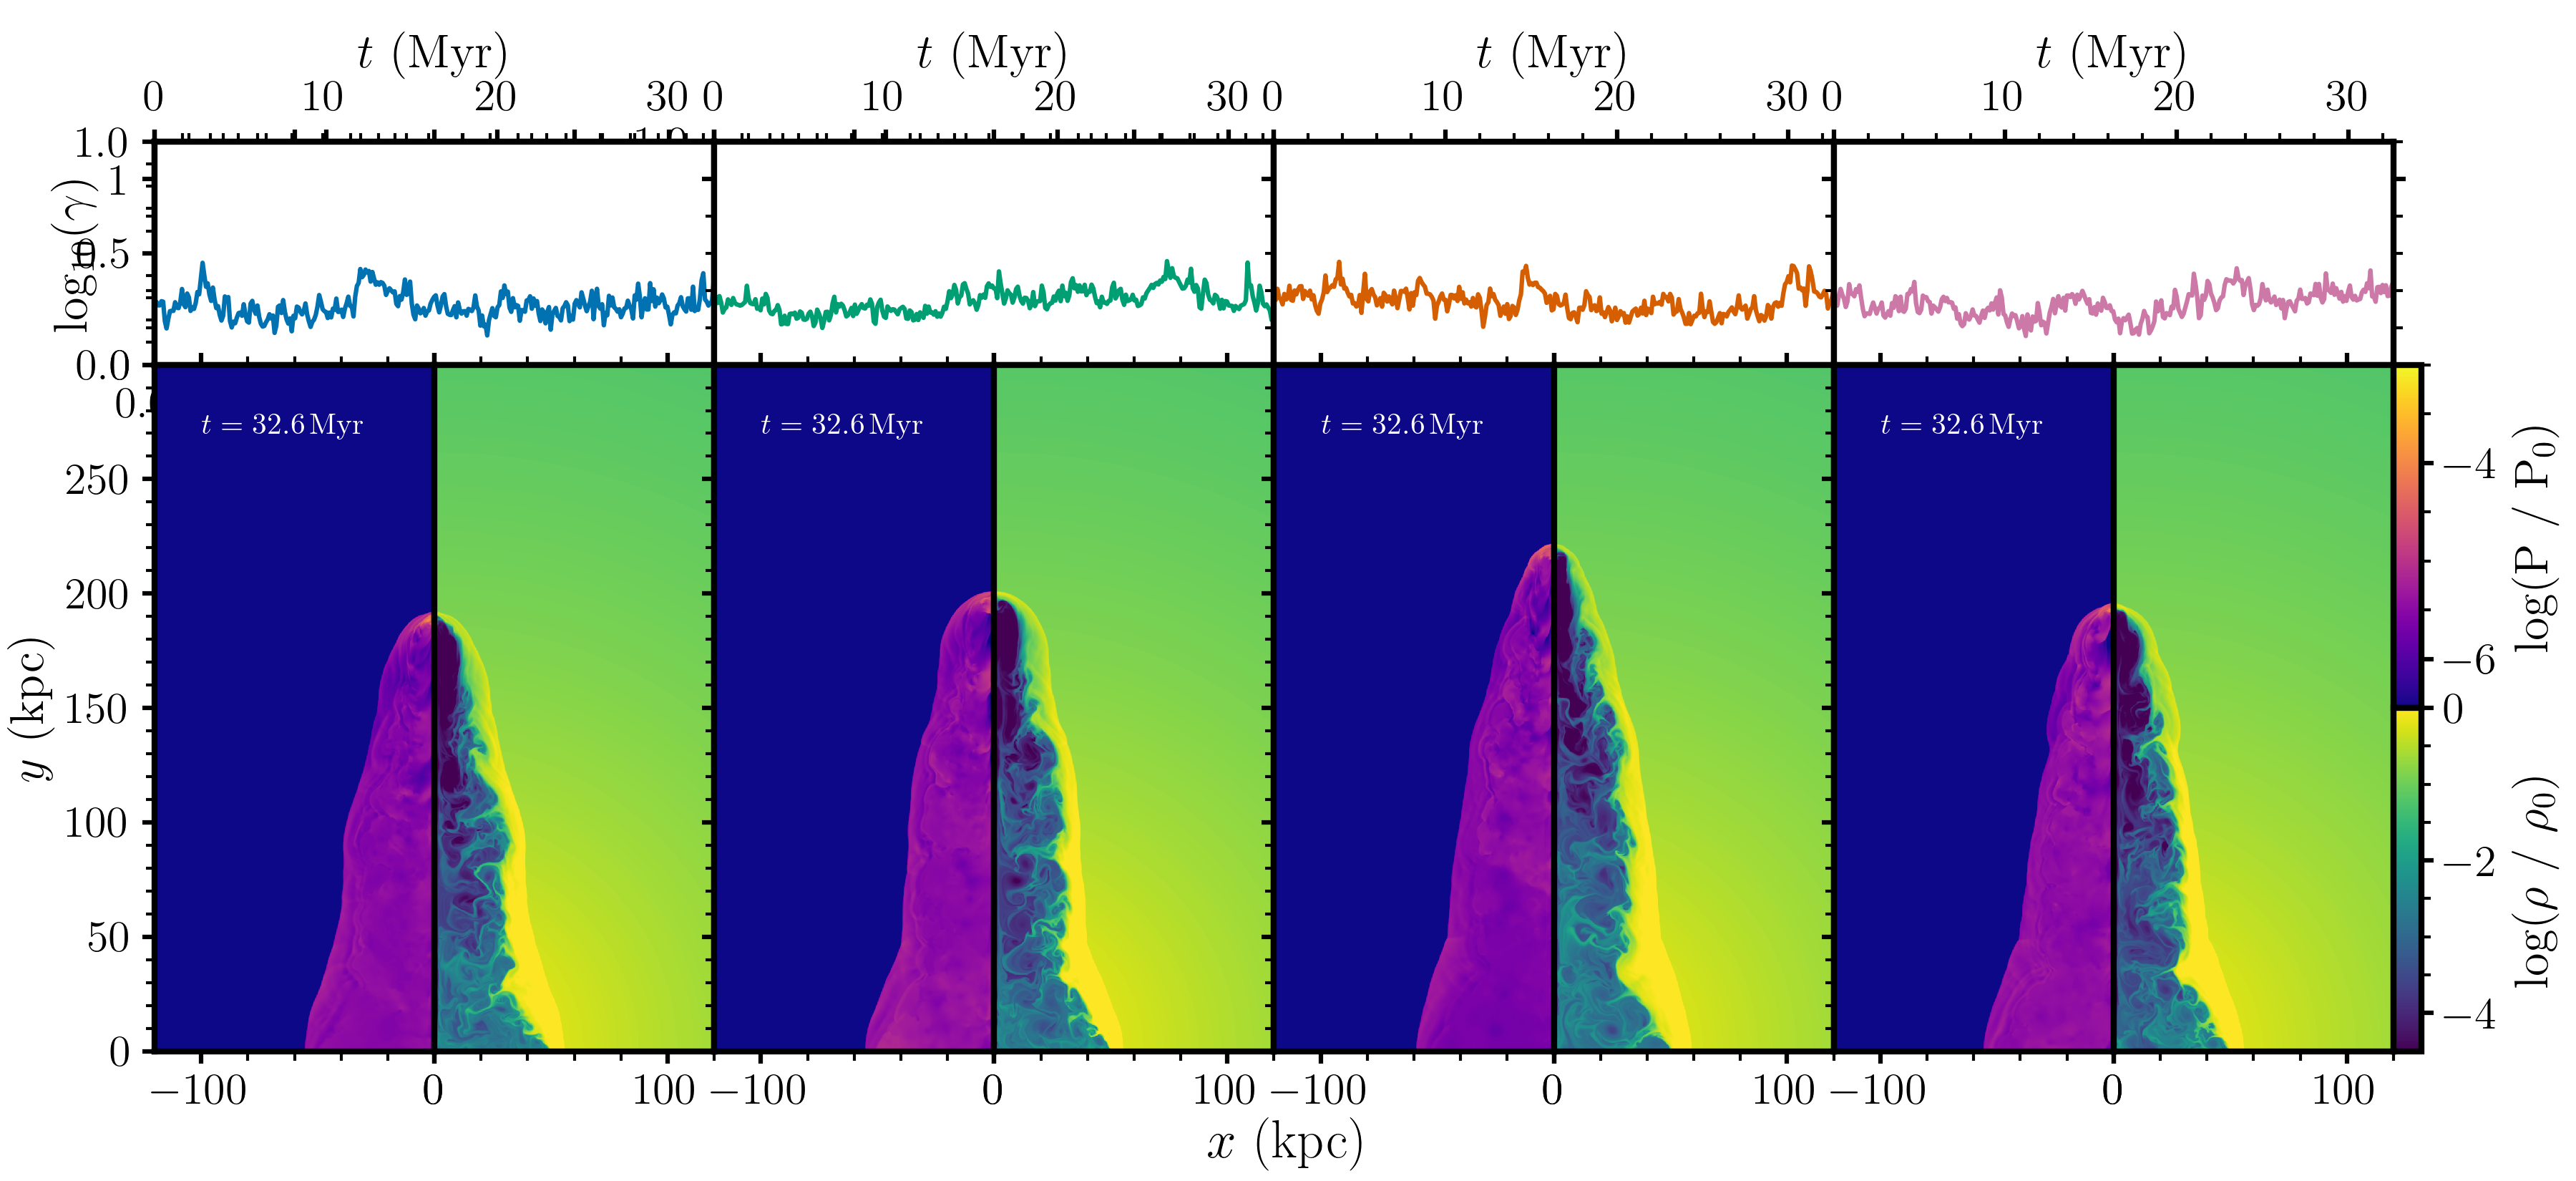
\includegraphics[width=0.97\linewidth]{quad05.png}
    \caption{
    As Fig.~3, but for $\sigma=0.5$.
    }
    \label{fig:4panel_sigma0.5}
\end{figure*}

\begin{figure*}
    \centering
    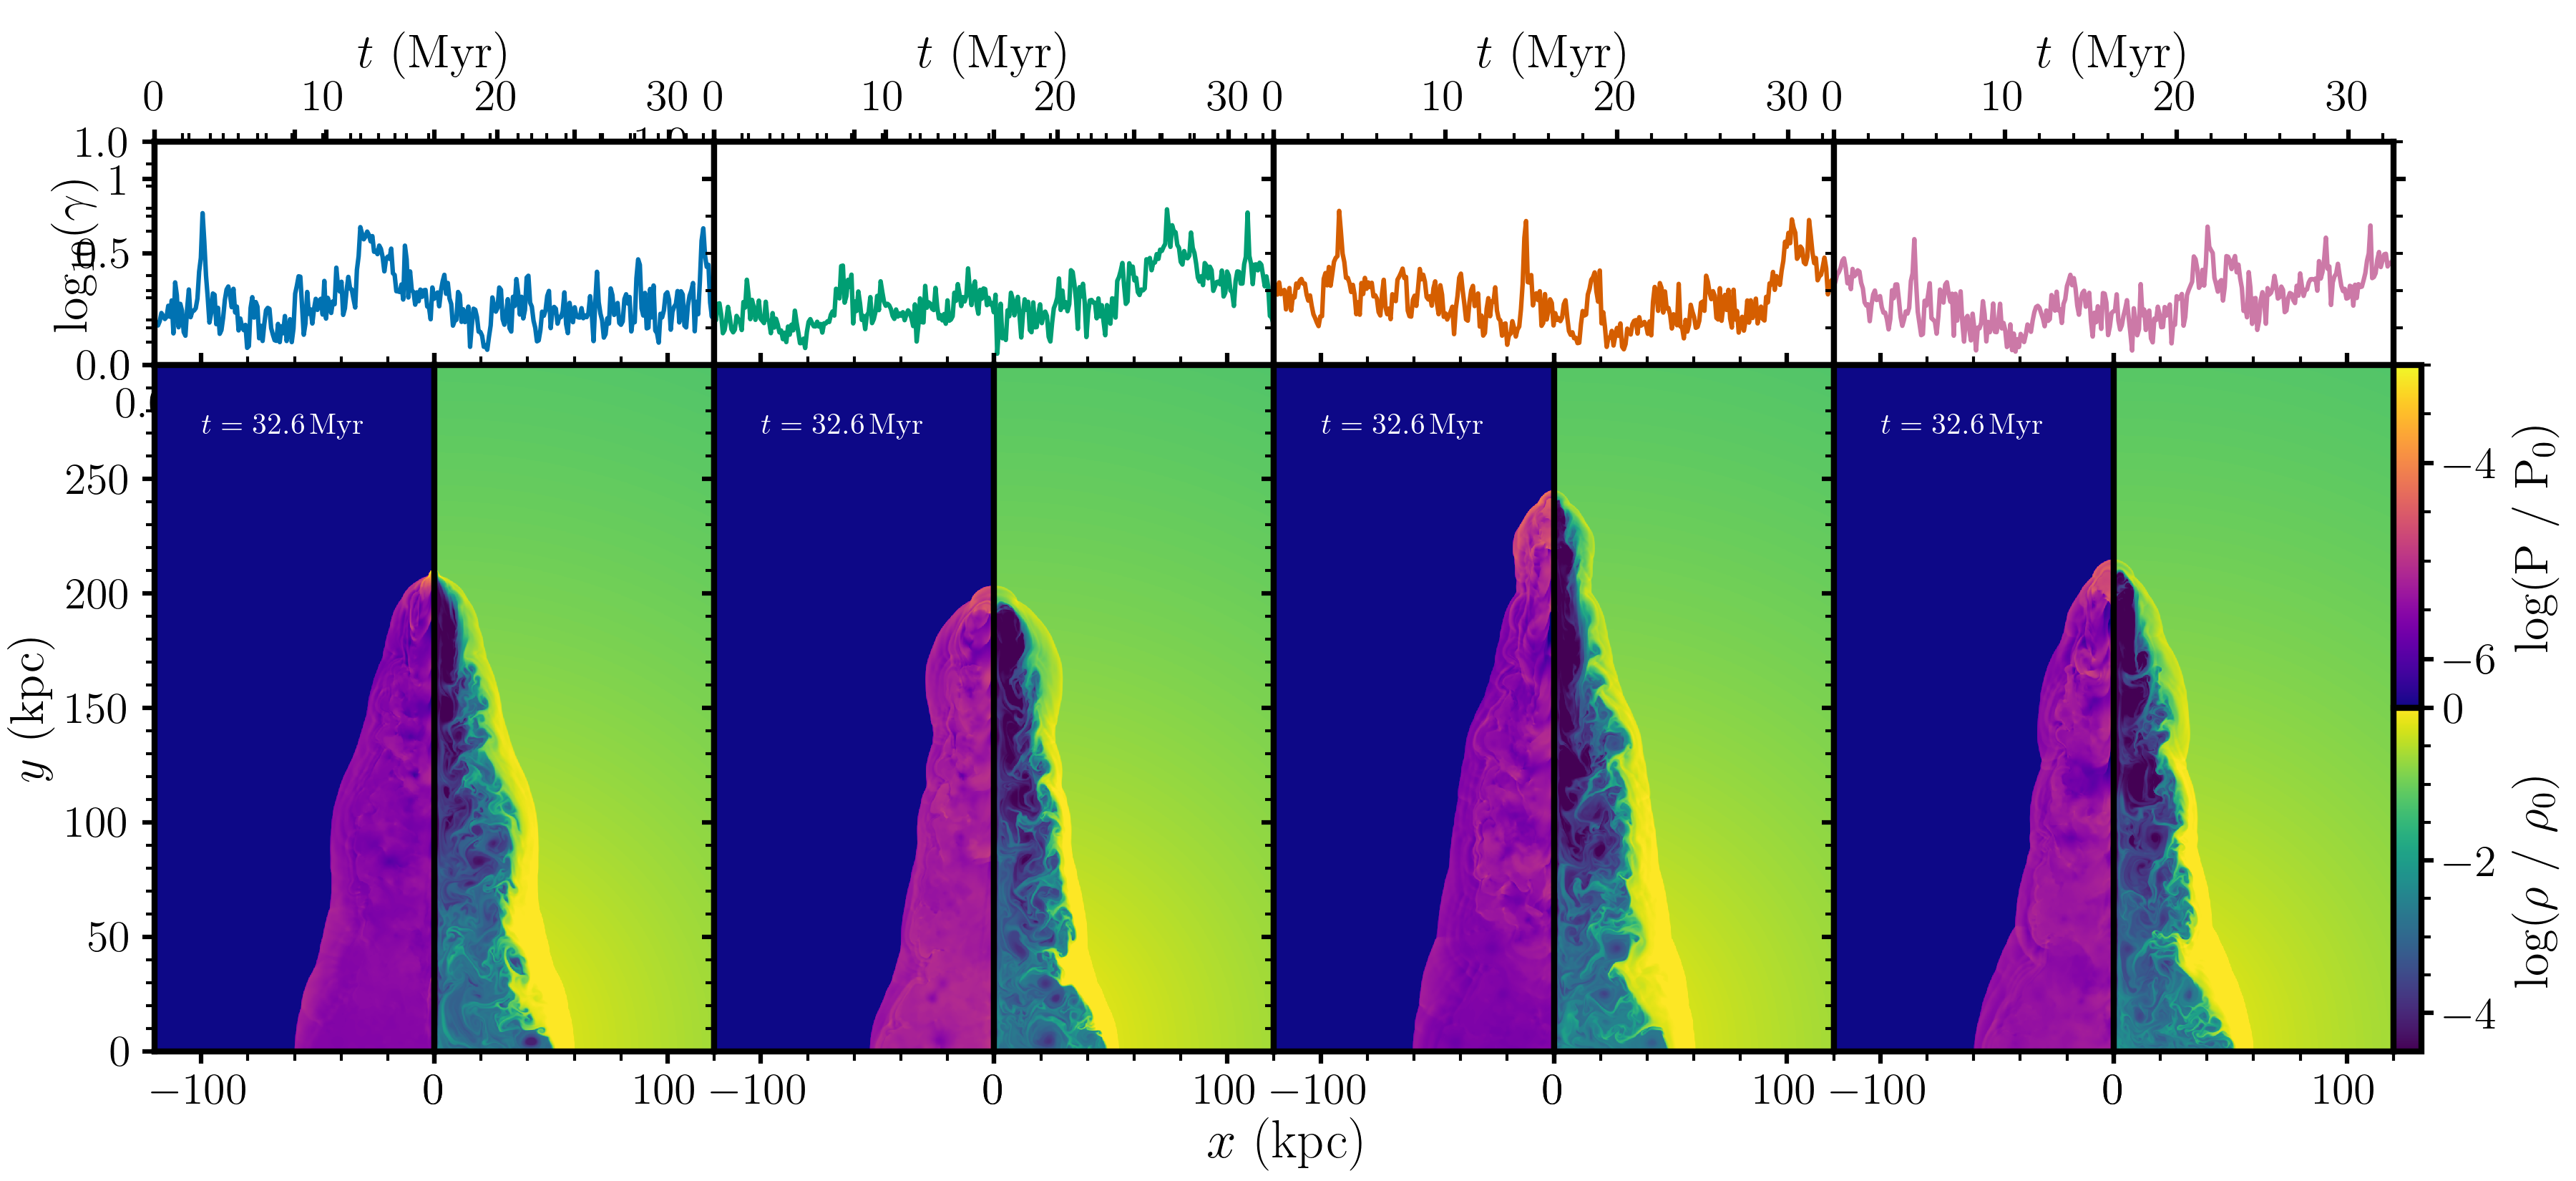
\includegraphics[width=0.97\linewidth]{quad1.png}
    \caption{
    As Fig.~3, but for $\sigma=1$.
    }
    \label{fig:4panel_sigma1}
\end{figure*}

\begin{figure*}
    \centering
    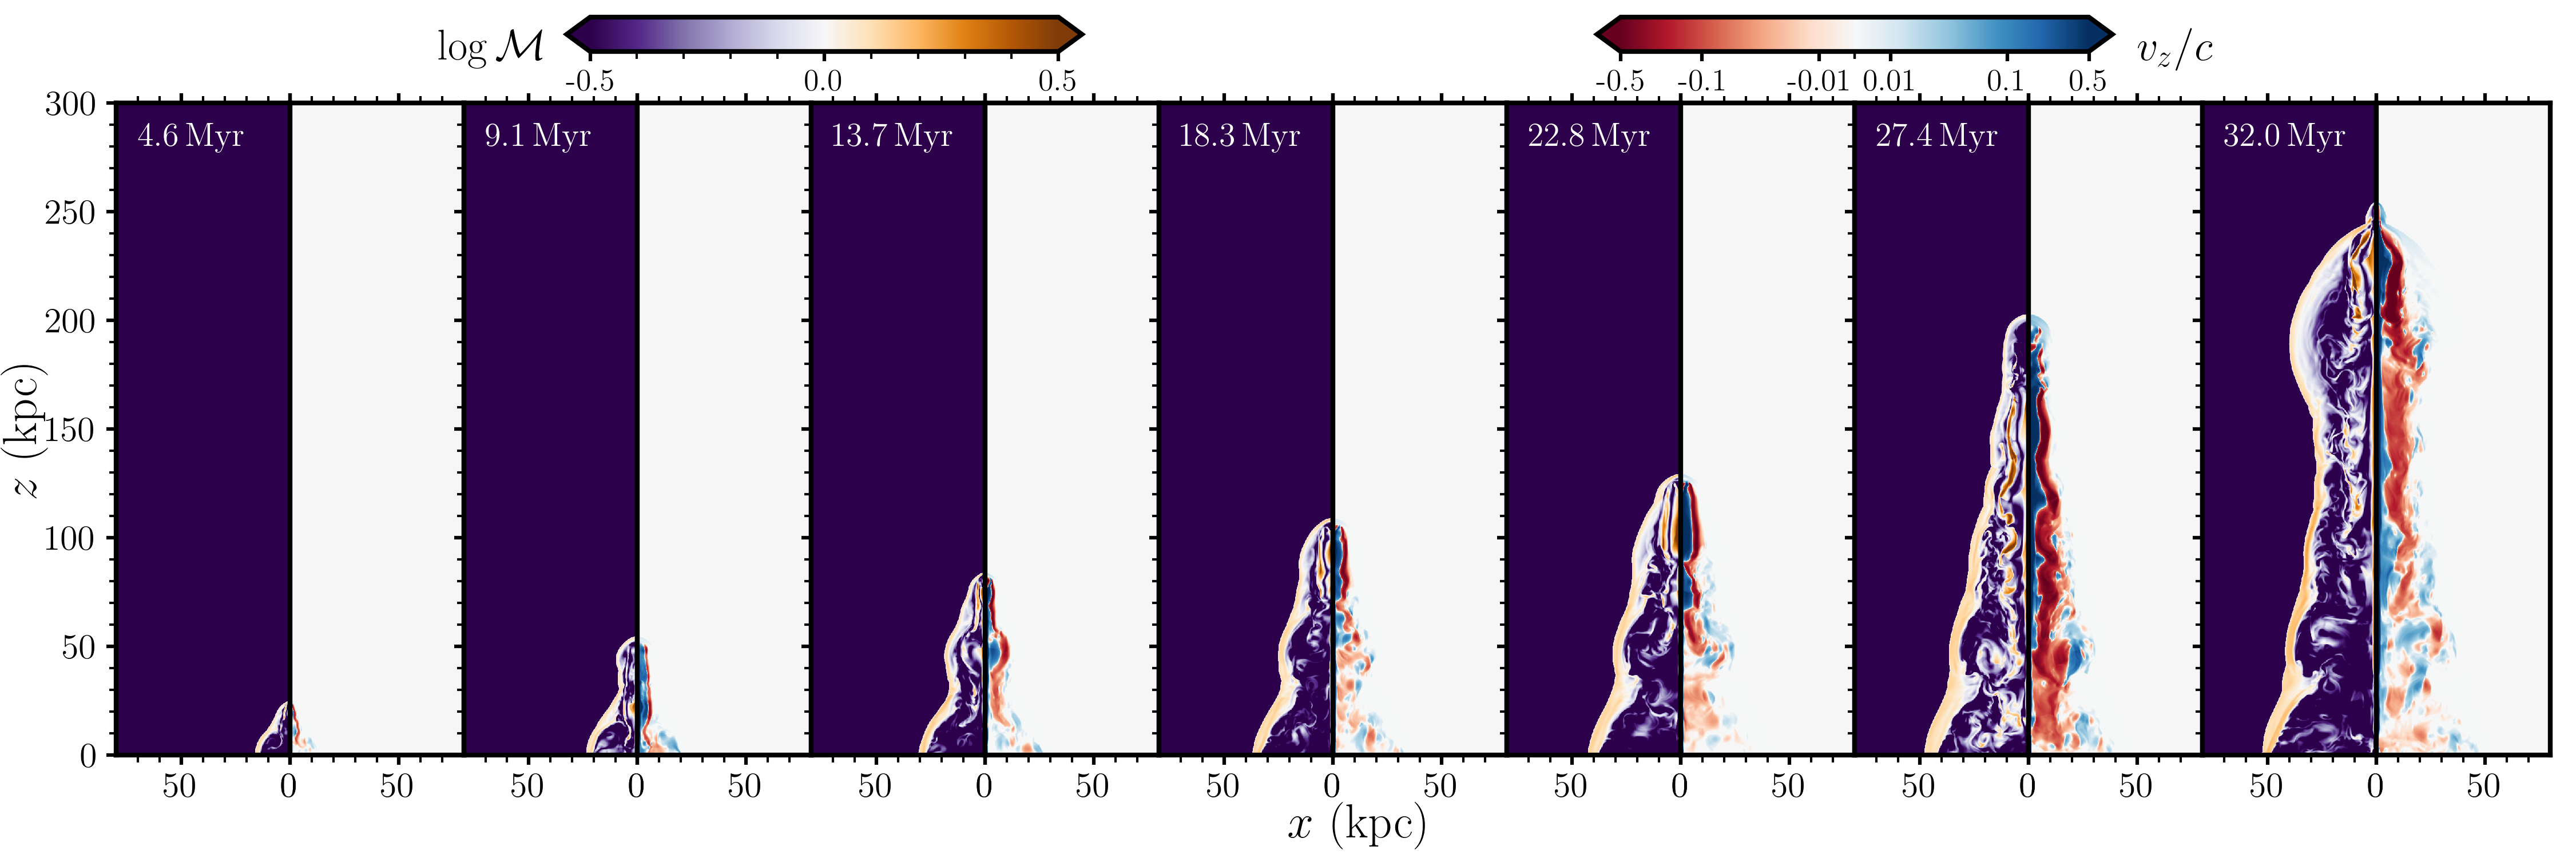
\includegraphics[width=0.97\linewidth]{ColorMeshTime_40.png}
    \caption{
    As Fig.~7, but for a different RNG seed ($i=40$).
    }
    \label{fig:ColorMeshTime_40}
\end{figure*}

\begin{figure*}
    \centering
    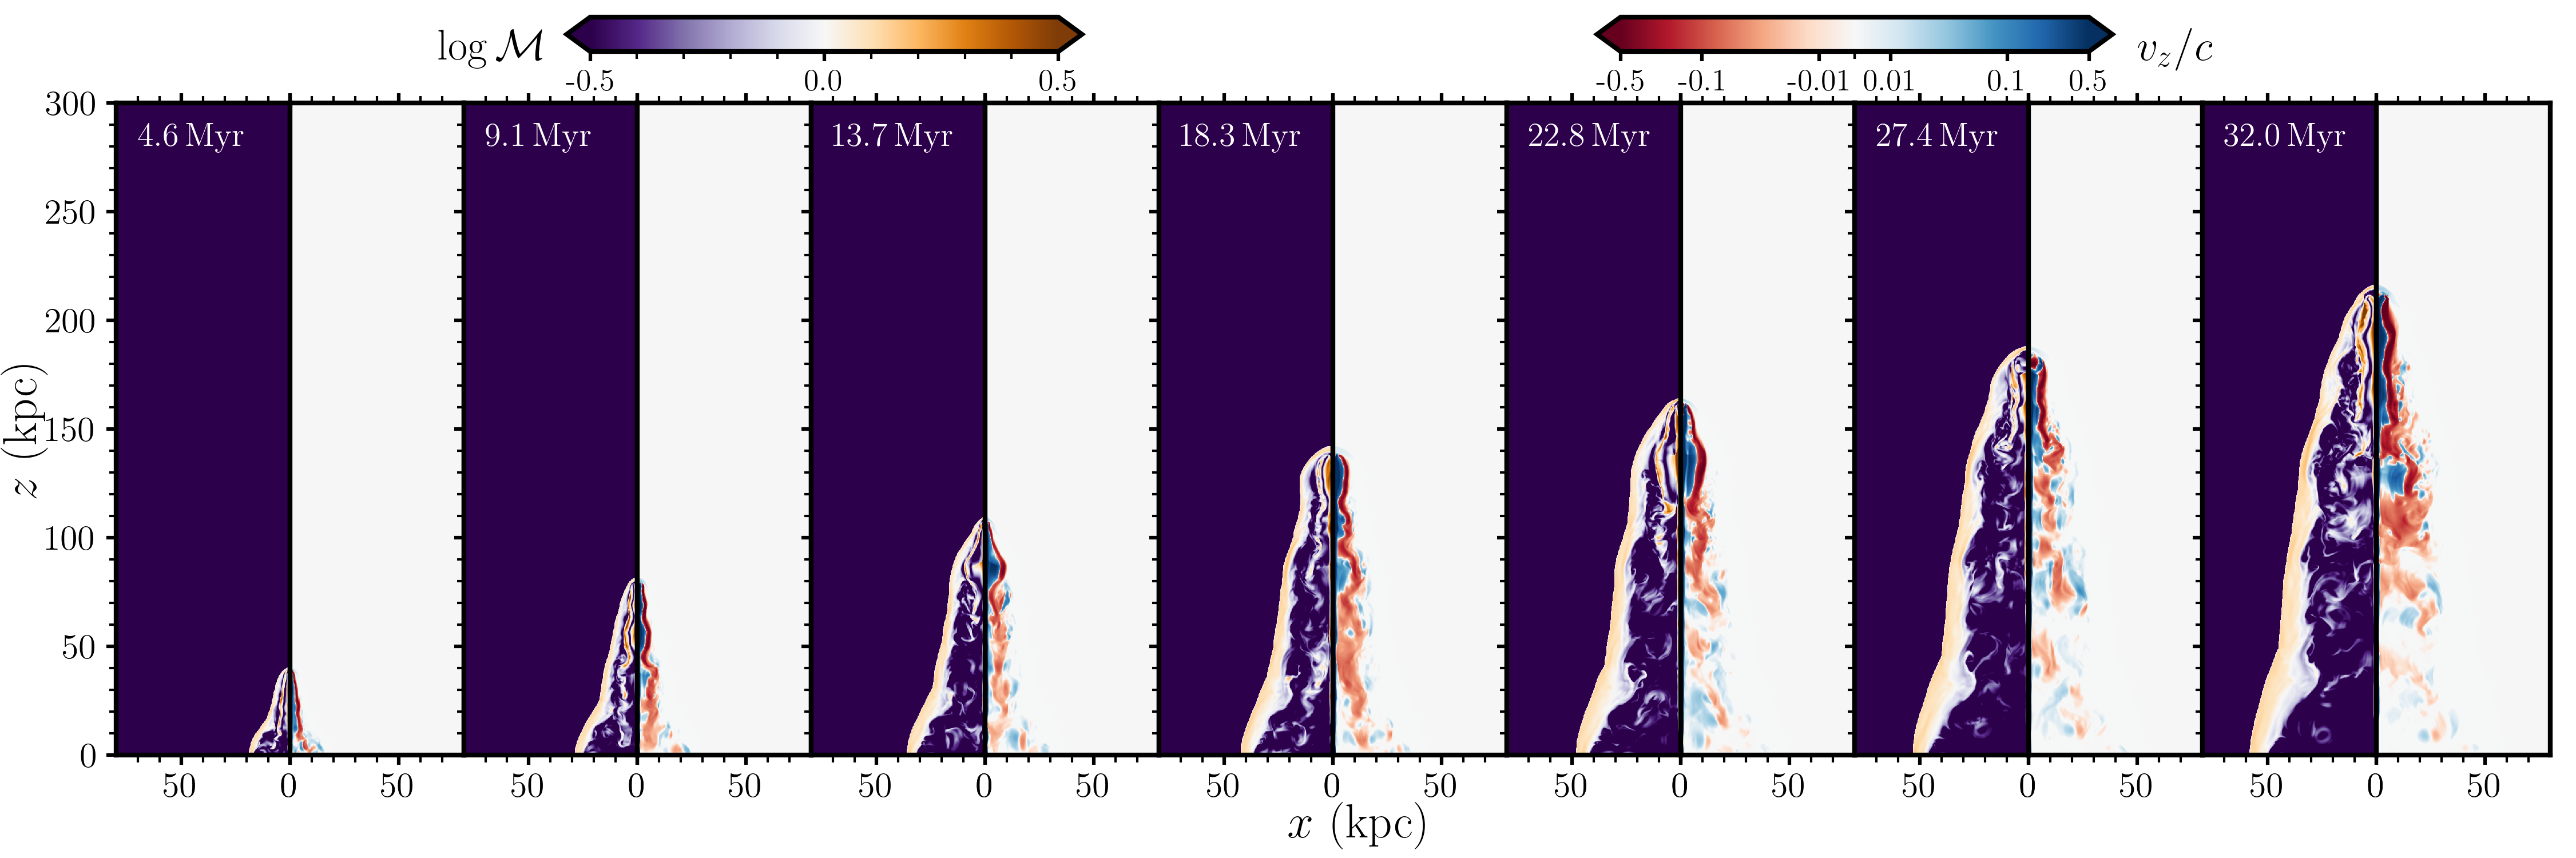
\includegraphics[width=0.97\linewidth]{ColorMeshTime_sig05.png}
    \caption{
    As Fig.~7, but for $\sigma=0.5$.
    }
    \label{fig:ColorMeshTime_05}
\end{figure*}

\begin{figure*}
    \centering
    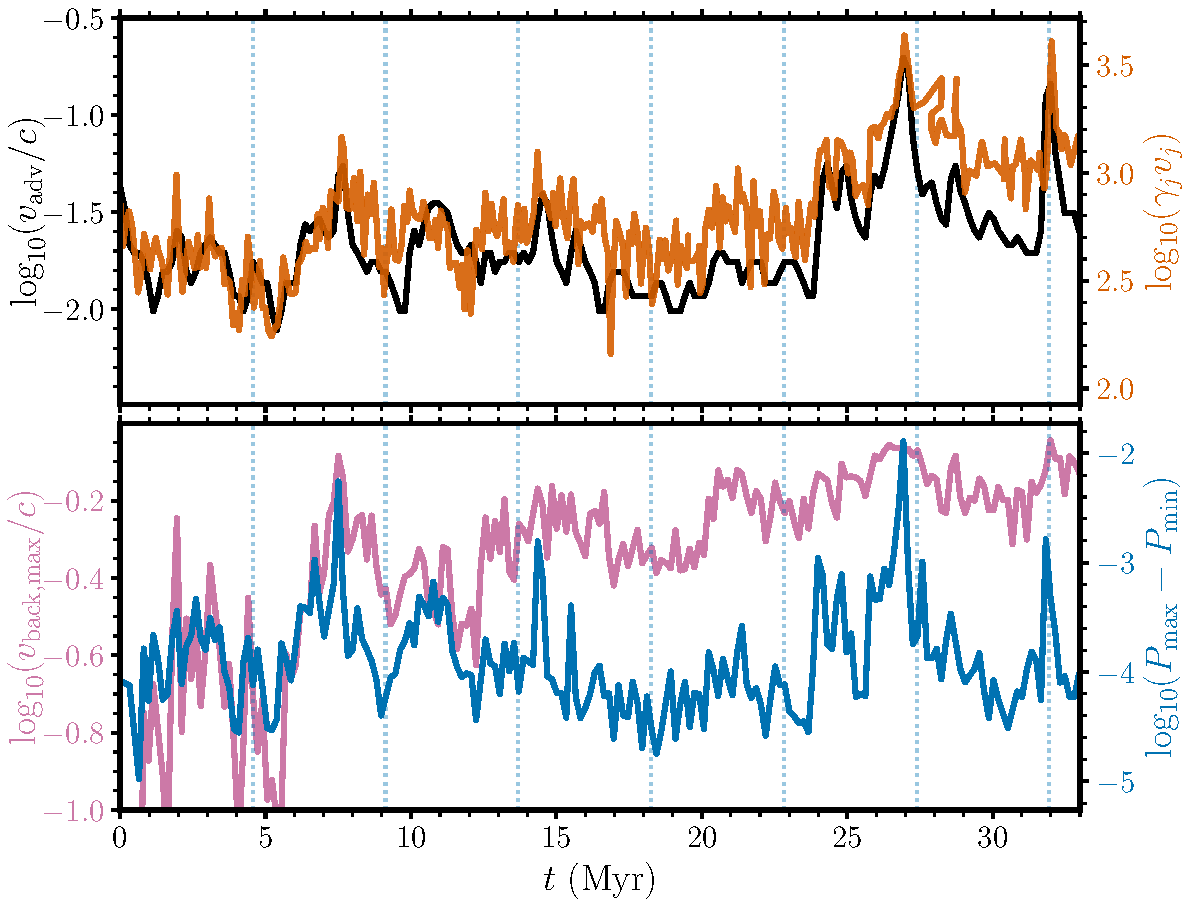
\includegraphics[width=0.48\linewidth]{advance_with_backflow_sig1.5_seed40.pdf}
    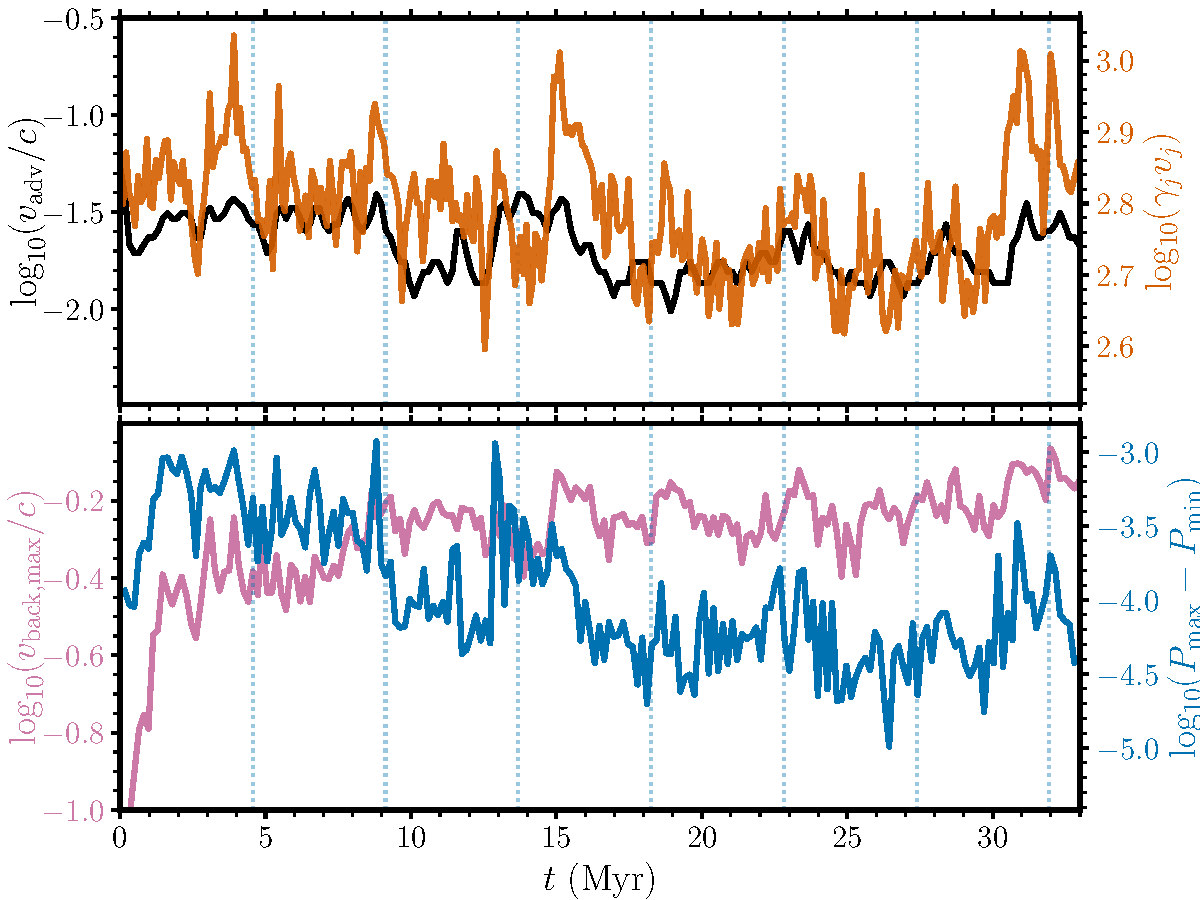
\includegraphics[width=0.48\linewidth]{advance_with_backflow_sig0.5_seed43.pdf}
    \caption{
    As Fig.~8, but for $i=40$ (left) and $\sigma=0.5$ (right).
    }
    \label{fig:backflow_other_seeds}
\end{figure*}

% Don't change these lines
\bsp    % typesetting comment
\label{lastpage}
\end{document}